\section{Context-free Grammars}
Context-free grammars (CFGs) are a method for describing syntactical composition of sentences in a language.
It does not describe the meaning of the sentences, hence the name, "context-free".
CFGs split sentences into "terminals" and "non-terminals" (also known as variables).
A terminal is the most basic structure of a sentence, and consists only of characters from the language's alphabet.
Terminals are most often written using camelCase.
A non-terminal is a superstructure that can consist of both terminals and non-terminals, or an empty string.
The same non-terminal can point to different structures.
Non-terminals are most often written using PascalCase.
%INSERT SOURCE

Although the concept of CFGs was originally meant to be used to describe sentence structure in languages such as English, they have proven useful in doing the same for strings in programming languages.
%INSERT SOURCE

The box below showcases how a language can be described using CFGs.
\begin{align*}
	\texttt{Sentence}\to & \texttt{ StringOfWords \$}\\
	\texttt{StringOfWords}\to & \texttt{ "word" StringOfWords}\\
	| & \texttt{ }\lambda
\end{align*}

The grammar contains:
\begin{itemize}
	\item two non-terminals, "Sentence" and "StringOfWords",
	\item one terminal, "word",
	\item the empty string (denoted by a lambda, $\lambda$),
	\item and a dollar-sign, \$, marking the end of the string.
\end{itemize}

The rules of the grammar are as follows:

Sentence consists of one StringOfWords. 
A StringOfWords consists of the string "word" followed by another StringOfWords, or an empty string.
As StringOfWords appears on the right-hand side of the arrow in its own definition, it is recursive.

\textbf{Parse trees} can be used to see if a string is in the language described by a CFG.
If a parse tree can be constructed from a string using the rules of the CFG, that string is in the language described by the CFG. 
In a parse tree, the leaves are terminals and the rest of the nodes are non-terminals.
Figure \ref{} shows an example of a parse tree for a string in the grammar above.

\begin{figure}[H]
	\centering
	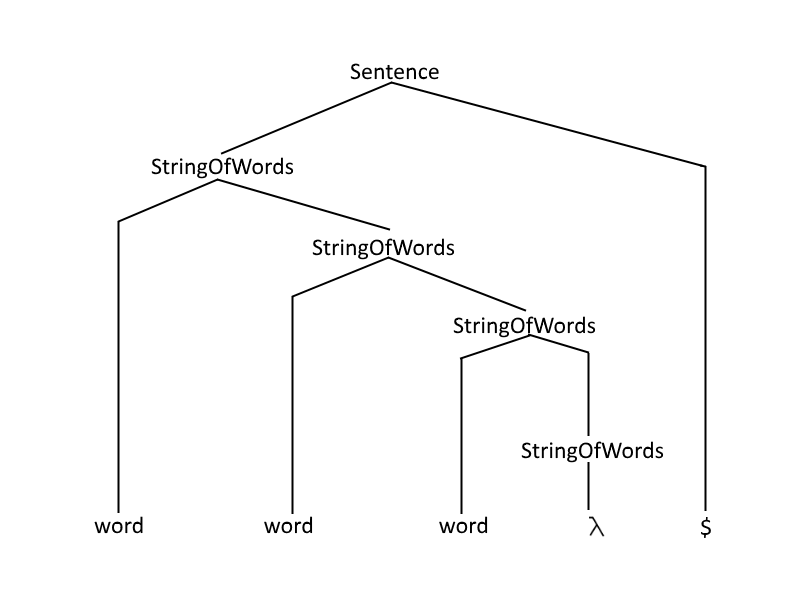
\includegraphics[width=\textwidth/2+\textwidth/4]{3.Theory/images/ParseTree.png}
	\caption{Parse tree for the string "word word word".}
	\label{fig:ParseTreeEx}
\end{figure}

Parse trees can be traversed using Depth First Search (DFS).

\textbf{Ambiguity} is when a string can be represented with two or more different parse trees using the same CFG.
It's a problem if a compiler is built from an ambiguous grammar, as a statement can be interpreted in different ways by the compiler.
The following is an example of an ambiguous grammar:
\begin{align*}
	\texttt{AssignStatement}\to & \texttt{ identifier = Expression}\\
	\texttt{Expression}\to & \texttt{ Expression + Expression}\\
	| & \texttt{ Expression * Expression}\\
	| & \texttt{ number}
\end{align*}

At first glance the grammar seems to accurately describe an assignment to a variable, but it does not describe the order of which the expression non-terminals are evaluated.
This means that a compiler which uses this grammar can give unintended results, and two compilers using the same CFG can create two different parse trees.
Below is an example of an ambiguous string using this CFG.
Figure \ref{fig:AmbiguousGrammarEx1} and figure \ref{fig:AmbiguousGrammarEx2} show two different parse

\texttt{x = 4 + 5 * 6 + 12}

\begin{figure}[H]
	\centering
	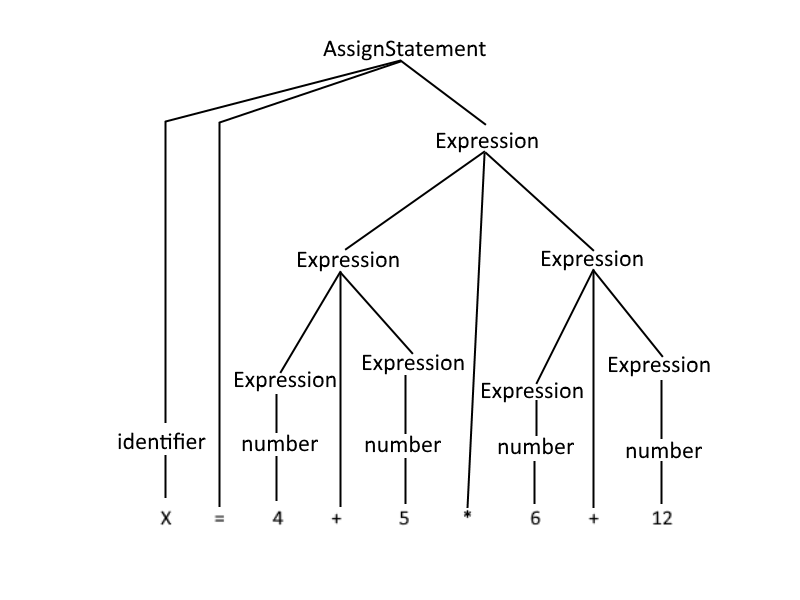
\includegraphics[width=\textwidth/2+\textwidth/4]{3.Theory/images/AmbiguousGrammar1.png}
	\caption{One parse tree for the string. The resulting value of x after a DFS traversal is 162.}
	\label{fig:AmbiguousGrammarEx1}
\end{figure}

\begin{figure}[H]
	\centering
	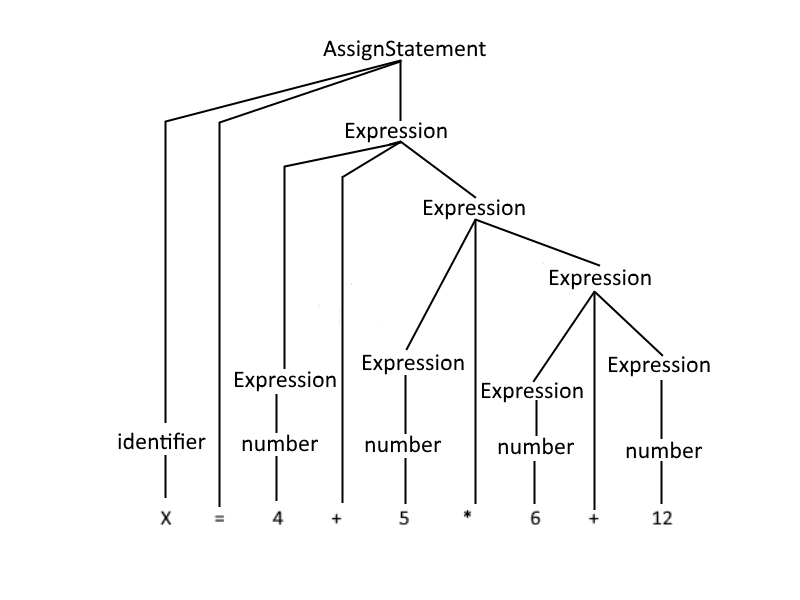
\includegraphics[width=\textwidth/2+\textwidth/4]{3.Theory/images/AmbiguousGrammar2.png}
	\caption{Another parse tree for the same string. The resulting value of x after a DFS traversal is 94.}
	\label{fig:AmbiguousGrammarEx2}
\end{figure}

\textbf{Backus-Naur Form} (BNF) is another way to write CFGs, although it is almost identical to the previous way. The only notable difference is the notation for non-terminals, which are enclosed in brackets:
\begin{align*}
	\texttt{<Sentence>}\to & \texttt{ <StringOfWords> \$}\\
	\texttt{<StringOfWords>}\to & \texttt{ "word" <StringOfWords>}\\
	| & \texttt{ }\lambda
\end{align*}

\textbf{Extended BNF} (EBNF) is yet another way to write CFGs. As the name suggests it adds new "features" to the BNF.
It is designed to be more concise than BNF.
In BNF, if a non-terminal is structured in two or more different ways, each way has to be noted with a new rule (like the \texttt{Expression} non-terminal from earlier).
In EBNF the number of rules can be reduces.
This is done by marking repetitive and optional arguments as well as choice of arguments within that one rule.
%Ovenstående sætning er vildt svær at formulere :(

The notation for EBNF is as follows:
\begin{align*}
	\text{Repetition (zero or more):} & \texttt{ \{arg\}}\\
	\text{Repetition (one or more):} & \texttt{ \{arg\}+}\\
	\text{Optional (zero or one):} & \texttt{ [arg]}\\
	\text{Choice:} & \texttt{ (arg1 | arg2)}
\end{align*}

The grammar for sentences can be rewritten in EBNF as
\begin{align*}
	\texttt{<Sentence>}\to & \texttt{ \{"word"\} \$}
\end{align*}
Note that the StringOfWords non-terminal is not needed anymore.

The ambiguous grammar for assignment can be rewritten in EBNF as
\begin{align*}
	\texttt{<AssignStatement>}\to & \texttt{ identifier = number [(+ | *) number]}
\end{align*}
Here it should be noted that, because the Expression non-terminal is gone, this grammar is not ambiguous anymore.